%!TEX root = ../main.tex

%\section*{Abstract}
%Probabilistic proposals of Language of Thoughts (LoTs) can explain learning across different domains as statistical inference over a compositionally structured hypothesis space. While frameworks may differ on how a LoT may be implemented computationally, they all share the property that they are built from a set of atomic symbols and rules by which these symbols can be combined.
%In this work we propose an extra validation step for the set of atomic productions defined by the experimenter. It starts by expanding the defined LoT grammar for the cognitive domain with a broader set of arbitrary productions and then uses Bayesian inference to prune the productions from the experimental data. The result allows the researcher to validate that the resulting grammar still matches the intuitive grammar chosen for the domain. We then test this method in the \textit{language of geometry}, a specific LoT model for geometrical sequence learning. Finally, despite the fact of the geometrical LoT not being a universal (i.e. Turing-complete) language, we show an empirical relation between a sequence's {\em probability} and its {\em complexity} consistent with the theoretical relationship for universal languages described by Levin's Coding Theorem.

\chapter{Validación bayesiana de producciones gramaticales para el lenguaje del pensamiento}\label{chapter:PO}
\chaptermark{Validación bayesiana de gramáticas}


%Most studies of LoTs have focused on the compositional aspect of the language, which has either been modeled within a Bayesian~\cite{tenenbaum2011grow} or a Minimum Description Length (MDL) framework~\cite{amalric2017language,goldsmith2002probabilistic,romano2013language,goldsmith2001unsupervised}.

La mayoría de los estudios de \lot se han centrado en el aspecto compositivo del lenguaje, modelando la composición a través de técnicas de inferencia bayesiana~\cite{tenenbaum2011grow} o de longitud mínima de descripción (MDL)~\cite{amalric2017language,goldsmith2002probabilistic,romano2013language,goldsmith2001unsupervised}.

%The common method is to define a grammar with a set of productions based on operations that are intuitive to researchers and then study how different inference processes match regular patterns in human learning. A recent study~\cite{piantadosi2016logical} puts the focus on the process of how to empirically choose the set of productions and how different LoT definitions can create different patterns of learning. Here, we move along that direction but use Bayesian inference to individuate the LoT instead of comparing several of them by hand.

El método más común es definir una gramática con un conjunto de producciones basadas en operaciones que son intuitivas para los investigadores y luego estudiar cómo diferentes procesos de inferencia coinciden con los patrones del aprendizaje humano. Un estudio reciente~\cite{piantadosi2016logical} pone el foco en el proceso de cómo elegir empíricamente el conjunto de producciones y cómo diferentes definiciones del \lot pueden crear diferentes patrones de aprendizaje. En este capítulo, encaramos esa dirección pero utilizando la inferencia bayesiana para seleccionar el \lot en lugar de seleccionarlo a partir de la comparación empírica de las distintas versiones con los patrones a replicar.


%Broadly, our aim is to propose a method to select the set of atomic symbols in an inferential process by pruning and trimming from a broad repertoire. More precisely, we test whether Bayesian inference can be used to decide the proper set of productions in a LoT defined by a context free grammar. These productions are derived from the subjects' experimental data. In order to do this, a researcher builds a broader language with two sets of productions: 1) those for which she has a strong prior conviction that they should be used in the cognitive task, and 2) other productions that could be used to structure the data and extract regularities even if she believes are not part of the human reasoning repertoire for the task. With the new broader language, she should then turn the context free grammar that defines it into a probabilistic context free grammar (PCFG) and use Bayesian analysis to infer the probability of each production in order to choose the set that best explains the data.

En términos generales, nuestro objetivo es proponer un método para seleccionar el conjunto de símbolos atómicos en un proceso de inferencia, seleccionándolos y recortándolos de un repertorio más amplio. Más precisamente, nos interesa probar si la inferencia bayesiana puede utilizarse para decidir el conjunto adecuado de producciones en un \lot definido por una gramática libre de contexto, derivando las producciones a elegir de los datos experimentales de los sujetos del experimento. Para hacer esto, un investigador debería construir un lenguaje suficientemente amplio con dos conjuntos de producciones: 1) aquellas para las que tiene una fuerte convicción previa de que podrían ser utilizadas en la tarea cognitiva a estudiar, y 2) otras producciones que podrían utilizarse para estructurar los datos y extraer regularidades incluso si cree que no son parte del repertorio de razonamiento humano para la tarea. Con el nuevo lenguaje más amplio, debería convertir la gramática libre de contexto que lo define en una gramática libre de contexto probabilística (PCFG) y utilizar el análisis bayesiano para inferir la probabilidad de cada producción y, así, el conjunto que mejor explique los datos.

%In the next section we formalize this procedure and then apply it on the \textit{language of geometry} presented by Amalric et al. in a recent study about geometrical sequence learning~\cite{amalric2017language}. This LoT defines a language with some basic geometric instructions as the grammar productions and then models their composition within the MDL framework. Our method, however, can be applied to any LoT model that defines a grammar, independently of whether its compositional aspect is modeled using a Bayesian framework or a MDL approach.

En la siguiente sección, formalizaremos este procedimiento, que luego lo aplicaremos en la gramática \gramgeo. Nuestro método, sin embargo, se puede aplicar a cualquier modelo de \lot que defina una gramática, independientemente de si su aspecto compositivo se modela utilizando un enfoque de probabilidad bayesiana o de MDL.

%Finally, even with the recent surge of popularity of Bayesian inference and MDL in cognitive science, there are --to the best of our knowledge-- no practical attempts to close the gap between probabilistic and complexity approaches to LoT models.

Finalmente, incluso con el reciente aumento de popularidad de la inferencia bayesiana y el MDL en la ciencia cognitiva, no hay --hasta donde sabemos-- intentos prácticos de cerrar la brecha entre ambos enfoques.

%The theory of computation, through Levin's Coding Theorem~\cite{levin1974laws}, exposes a remarkable relationship between the {\em Kolmogorov complexity} of a sequence and its {\em universal probability}, largely used in algorithmic information theory. Although both metrics are actually non-computable and defined over a universal prefix Turing Machine, we can apply both ideas to other non-universal Turing Machines in the same way that the concept of complexity used in MDL can be computed for specific, non-universal languages.

La teoría de la computabilidad, a través del Teorema de Codificación de Levin~\cite{levin1974laws}, expone una notable relación entre la {\em complejidad de Kolmogorov} de una secuencia (que es la base del cálculo del MDL) y su {\em probabilidad universal}, la cual es ampliamente utilizada en la teoría algorítmica de la información. Aunque ambas métricas resultan no computables y se encuentran definidas sobre una máquina Universal de Turing libre de prefijos, podemos aplicar estas ideas a otras máquinas de Turing no universales de la misma manera que el concepto de complejidad es utilizado para el cálculo de MDL en lenguajes específicos no universales. 

%In this work, we examine the extent to which this theoretical prediction for infinite sequences holds empirically for a specific LoT, the \textit{language of geometry}. Although the inverse logarithmic relationship between both metrics is proved for universal languages in the Coding Theorem, testing this same property for a particular non-universal language shows that the language shares some interesting properties of general languages. This constitutes a first step towards a formal link between probability and complexity modeling frameworks for LoTs.

En este trabajo también examinamos hasta qué punto esta predicción teórica para secuencias infinitas se preserva empíricamente para un \lot específico: \gramgeo. Aunque la relación logarítmica inversa entre ambas métricas está probada para lenguajes universales en el Teorema de Codificación, probar esta misma propiedad para un lenguaje no universal particular muestra que el lenguaje comparte algunas propiedades interesantes con los lenguajes generales. Esto constituye un primer paso hacia un vínculo formal entre el modelado de probabilidad y el de complejidad para el \lot.

%\section{Bayesian inference for LoT's productions}
\section{Inferencia bayesiana para las producciones del \lot}

%The project of Bayesian analysis of the LoT models concept learning using Bayesian inference in a grammatically structured hypothesis space~\cite{goodman2008rational}. Each LoT proposal is usually formalized by a context free grammar $\gram$ that defines the valid functions or programs that can be generated, like in any other programming language. A program is a derivation tree of $\gram$ that needs to be interpreted or executed according to a given semantics in order to get an actual description of the concept in the cognitive task at hand. Therefore, each concept is then represented by any of the programs that describe it and a Bayesian inference process is defined in order to infer from the observed data the distribution of valid programs in $\gram$ that describes the concepts.

El proyecto de análisis bayesiano del \lot modela el aprendizaje de conceptos utilizando la inferencia bayesiana en un espacio de hipótesis estructurado a partir de una gramática~\cite{goodman2008rational}. Cada propuesta de \lot suele formalizarse mediante una gramática libre de contexto $\gram$ que define las funciones o programas válidos que se pueden generar, como en cualquier otro lenguaje de programación. Aquí, un programa es un árbol de derivación de $\gram$ que necesita ser interpretado o ejecutado de acuerdo a una semántica dada para obtener una descripción real del concepto en la tarea cognitiva en cuestión. Por lo tanto, cada concepto puede ser representado por cualquiera de los programas que lo describen al ejecutarse, y un proceso de inferencia bayesiano es definido para calcular la distribución de los programas válidos de $\gram$ que describen los conceptos a explicar.

%As explained above, our aim is to derive the productions of $\gram$ from the data, instead of just conjecturing them using a priori knowledge about the task. Prior work on LoTs has fit probabilities of productions in a context free grammar using Bayesian inference, however, the focus has been put in integrating out the production probabilities to better predict the data without changing the grammar definition~\cite{piantadosi2016logical}. Here, we want to study if the inference process could let us decide which productions can be safely pruned from the grammar. We introduce a generic method that can be used on any grammar to select and test the proper set of productions. Instead of using a fixed grammar and adjusting the probabilities of the productions to predict the data, we use Bayesian inference to rule out productions with probability lower than a certain threshold. This allows the researcher to validate the adequacy of the productions she has chosen for the grammar or even define one that is broad enough to express different regularities and let the method select the best set for the observed data.

Como se explicó anteriormente, nuestro objetivo es derivar las producciones de $\gram$ a partir de los datos, en lugar de sólo conjeturarlas utilizando un conocimiento a priori sobre la tarea. Otros trabajos previos en \lot ajustaron las probabilidades de las producciones de las gramáticas libres de contexto utilizando inferencia bayesiana~\cite{piantadosi2016logical}, sin embargo, han puesto el foco en la integración de las probabilidades de producción para predecir mejor los datos y no en cambiar la definición de las gramáticas. Aquí queremos estudiar si el proceso de inferencia podría permitirnos decidir qué producciones de la gramática pueden podarse con seguridad. Para esto, introducimos un método genérico que puede utilizarse en cualquier gramática para seleccionar y probar el conjunto adecuado de producciones. En lugar de usar una gramática fija y ajustar las probabilidades de las producciones para predecir los datos, utilizamos la inferencia bayesiana para remover las producciones con una probabilidad inferior a cierto umbral. Esto permite al investigador validar la adecuación de las producciones que ha elegido para la gramática o incluso definir una que sea lo suficientemente amplia como para expresar diferentes regularidades y dejar que el método seleccione el mejor conjunto a partir de los datos observados.   


%To infer the probability for each production based on the observed data, we need to add a vector of probabilities $\theta$ associated with each production in order to convert the context free grammar $\gram$ into a probabilistic context free grammar (PCFG)~\cite{manning1999foundations}.

Para inferir la probabilidad de cada producción a partir de los datos observados, necesitamos agregar un vector de probabilidades $\theta$ asociado con cada producción para convertir a la gramática libre de contexto $\gram$ en una gramática libre de contexto probabilística~\cite{manning1999foundations}.

%Let $D = (d_1, d_2, \dots, d_n)$ denote the list of concepts produced by the subjects in an experiment. This means that each $d_i$ is a concept produced by a subject in each trial. Then, $P(\theta \mid D)$, the posterior probability of the weights of each production after the observed data, can be calculated by marginalizing over the possible programs that compute $D$:

Sea $D = (d_1, d_2, \dots, d_n)$ la lista de conceptos obtenida de los sujetos en un experimento. Esto significa que cada $d_i$ es un concepto generado por un sujeto en cada ensayo. Luego, $P(\theta \mid D)$, la probabilidad a posteriori de los pesos de cada producción después de observar los datos, se puede calcular marginalizando sobre los posibles programas que computan $D$:
%
\begin{equation*}
\label{eqA}
P(\theta \mid D) = \sum_{\Prog } P(\Prog,\theta \mid D),
\end{equation*} donde cada $\Prog  = (p_1, p_2, \cdots, p_n)$ es un posible conjunto de programas tales que cada $p_i \in \gram$ computa el correspondiente concepto $d_i$ a partir de la semántica definida para la gramática, es decir, $\sem{p_i} = d_i$
%where each $\Prog  = (p_1, p_2, \cdots, p_n)$ is a possible set of programs such that each $p_i$ computes the corresponding concept $d_i$.

%We can use Bayesian inference to learn the corresponding programs $\Prog$ and the vector $\theta$ for each production in the grammar, applying Bayes rule in the following way:
Podemos usar la inferencia bayesiana para aprender los programas correspondientes $\Prog$ y el vector $\theta$ para cada producción de la gramática, aplicando la regla de Bayes de la siguiente manera:
%
\begin{equation}
\label{eq:mainB}
P(\Prog,\theta \mid D) \propto P(D \mid \Prog)\ P(\Prog \mid \theta)\ P(\theta).
\end{equation}
%

%Sampling the set of programs from $P(\Prog \mid \theta)$ forces an inductive bias which is needed to handle uncertainty under sparse data. Here we use a standard prior for programs that is common in the LoT literature to introduce a syntactic complexity bias that favors shorter programs~\cite{goodman2008rational,overlan2017learning}. Intuitively, the probability of sampling a certain program is proportional to the product of the production rules that were used to generate such program, and therefore inversely proportional to the size of the derivation tree. Formally, it is defined as:

Hacer un muestreo del conjunto de programas de $P(\Prog \mid \theta)$ fuerza un sesgo inductivo que es necesario para manejar la incertidumbre frente a datos escasos. Aquí usamos como probabilidad a priori para los programas un estándar que es común en la literatura de \lot para introducir un sesgo de complejidad sintáctica que favorece programas más cortos~\cite{goodman2008rational,overlan2017learning}. Intuitivamente, la probabilidad de muestreo de un determinado programa es proporcional al producto de las reglas de producción que se utilizaron para generar dicho programa y, por lo tanto, inversamente proporcional al tamaño del árbol de derivación. Formalmente, se define como:
%
\begin{equation*}
\label{eqC}
P(\Prog \mid \theta)\ = \prod\limits_{i = 1}^n P(p_i \mid \theta),
\end{equation*}
%
donde $P(p_i \mid \theta) = \prod\limits_{r \in \gram} \theta^{f_r(p_i)}_{r}$ es la probabilidad del programa $p_i$ en la gramática, y $f_r(p_i)$ es el número de ocurrencias de la producción $r$ en el programa $p_i$.
%where $P(p_i \mid \theta) = \prod\limits_{r \in G} \theta^{f_r(p_i)}_{r}$ is the probability of the program $p_i$ in the grammar, and $f_r(p_i)$ is the number of occurrences of the production $r$ in program $p_i$.

%In \eqref{eq:mainB}, $P(\theta)$ is a Dirichlet prior over the productions of the grammar. By using the term $P(\theta)$ we are abusing notation for simplicity. The proper term would be $P(\theta \mid \alpha)$ to express a Dirichlet prior with $\alpha \in \mathbb{R}^\ell$ its associated concentration vector hyper-parameter where $\ell$ is the number of productions in the grammar. This hierarchical Dirichlet prior has sometimes been replaced with a uniform prior on productions as it shows no significant differences in prediction results~\cite{piantadosi2012bootstrapping,yildirim2015learning}. However, here we will use the Dirichlet prior to be able to infer the production probabilities from this more flexible model.

En la ecuación \eqref{eq:mainB}, $P(\theta)$ es una Dirichlet que se utiliza como distribución a priori sobre las producciones de la gramática. Al utilizar el término $P(\theta)$ estamos abusando de la notación por simplicidad. El término adecuado sería $P(\theta \mid \alpha)$ para expresar la distribución a priori con $\alpha \in \mathbb{R}^\ell$ su hiperparámetro que actúa como vector de concentración asociado, donde $\ell$ es el número de producciones de la gramática. Esta distribución a proiri ha sido también reemplazada por una distribución uniforme, ya que no muestra diferencias significativas en resultados de predicción~\cite{piantadosi2012bootstrapping,yildirim2015learning}. Sin embargo, aquí utilizaremos la distribución Dirichlet para poder inferir las probabilidades de producción a partir de este modelo más flexible.

%The likelihood function is straightforward. It does not use any free parameter to account for perception errors in the observation. This forces that only programs that compute the exact concept are taken into account, and it can be easily calculated as follows:

La función de verosimilitud es sencilla. No utiliza ningún parámetro libre para contabilizar errores de percepción en la observación. Esto obliga a que sólo los programas que computan el concepto exacto se tengan en cuenta, y puede ser fácilmente calculada de la siguiente manera:
%
\begin{equation*}
\label{eqD}
P(D \mid \Prog)\ = \prod\limits_{i = 1}^n P(d_i \mid p_i),
\end{equation*}
%
%where $P(d_i \mid p_i) = 1 $ if the program $p_i$ computes $d_i$, and 0 otherwise.
donde $P(d_i \mid p_i) = 1 $ si $\sem{p_i} = d_i$ (el programa $p_i$ computa $d_i$), y 0 en caso contrario. 
%Calculating $P(\theta \mid D)$ directly is, however, not tractable since it requires to sum over all possible combinations of programs $\Prog$ for each of the possible values of $\theta$. To this aim, then, we used a Gibbs Sampling~\cite{geman1984stochastic} algorithm for PCFGs via Markov Chain Monte Carlo (MCMC) similar to the one proposed at~\cite{johnson2007bayesian}, which alternates in each step of the chain between the two conditional distributions:

Sin embargo, calcular $P(\theta \mid D)$ de manera directa no es computacionalmente tratable ya que requiere sumar todas las posibles combinaciones de programas $\Prog$ para cada uno de los posibles valores de $\theta$. Para este objetivo, utilizamos entonces el algoritmo de muestreo de Gibbs~\cite{geman1984stochastic} para PCFGs a través del Método de Monte Carlo basado en cadenas de Markov (MCMC, por sus siglas en inglés) similar al propuesto en~\cite{johnson2007bayesian}. Este método nos permite obtener una secuencia de muestras aleatorias para aproximar la distribución $P(\theta \mid D)$ a partir de la toma de muestras de manera alternada entre las distribuciones condicionales $P(\Prog \mid \theta, D)$ y $P(\theta \mid \Prog, D)$, las cuales sí pueden calcularse de manera directa. Dado que los algoritmos MCMC como este generan una secuencia de muestras donde cada una se correlaciona con muestras cercanas, las muestras del comienzo de la cadena suelen descartarse hasta que los valores se estabilizan (iteraciones de \textit{burn in}).
%
\begin{eqnarray*}
\label{eqE}
P(\Prog \mid \theta, D) &=& \prod\limits_{i=1}^n P(p_i \mid d_i, \theta),\\
P(\theta \mid \Prog, D) &=& P_D(\theta \mid f(\Prog) + \alpha).
\end{eqnarray*}
%Here, $P_D$ is the Dirichlet distribution where the positions of the vector $\alpha$ were updated by counting the occurrences of the corresponding productions for all programs $p_i \in \Prog$.
Aquí, $P_D$ es la distribución Dirichlet donde las posiciones del vector $\alpha$ fueron actualizadas contando las ocurrencias de las producciones correspondientes para todos los programas $p_i \in \Prog$.

%In the next section, we apply this method to a specific LoT. We add a new set of ad-hoc productions to the grammar that can explain regularities but are not related to the cognitive task. Intuitively, these ad-hoc productions should not be part of the human LoT repertory, still all of them can be used in many possible programs to express each concept.

En la siguiente sección, aplicamos este método a la gramática \gramgeo. Agregamos un nuevo conjunto ad-hoc de producciones a la gramática original que pueden explicar regularidades pero que no están relacionadas con la tarea cognitiva del problema original. Intuitivamente, estas producciones ad-hoc no deberían formar parte del repertorio de \gramgeo; aún así, todas ellas pueden usarse en muchos programas posibles para expresar cada uno de los conceptos.

%So far, Probabilistic LoT approaches have been successful to model concept learning from few examples~\cite{tenenbaum2011grow,piantadosi2016four}. However, this does not mean that Bayesian models would be able to infer the syntax of the model's grammar from sparse data. Here we test such hypothesis. If the method is effective, it should assign a low probability to the ad-hoc productions and instead favor the original set of productions selected by the researchers for the cognitive task. This would not only provide additional empirical evidence about the adequacy of the choice of the original productions for the selected LoT but, more importantly, about the usefulness of Bayesian inference for validating the set of productions involved in different LoTs.

Hasta ahora, los enfoques probabilísticos del \lot han tenido éxito para modelar el aprendizaje de conceptos a partir de pocos ejemplos~\cite{tenenbaum2011grow,piantadosi2016four}. Sin embargo, esto no significa que los modelos bayesianos puedan inferir la sintaxis de la gramática a partir de datos escasos. Aquí probamos esta hipótesis. Si el método es eficaz, debería asignar una probabilidad baja las producciones ad-hoc y en su lugar favorecer el conjunto original de producciones seleccionadas por los investigadores para la tarea cognitiva. Esto no sólo proporcionaría evidencia empírica adicional sobre la idoneidad de la elección original de producciones para el \lot, sino que --más importante-- brindaría evidencia sobre la utilidad de la inferencia bayesiana para validar el conjunto de producciones involucradas en diferentes LoTs. 

%\section{The Language of Geometry: $\gramgeo$}
\section{El lenguaje de geometría: \gramgeo}

%The \textit{language of geometry}, $\gramgeo$~\cite{amalric2017language}, is a probabilistic generator of sequences of movements on a regular octagon like the one in Figura~\ref{fig:circle}. It has been used to model human sequence predictions in adults, preschoolers, and adult members of an indigene group in the Amazon. As in other LoT domains, different models have been proposed for similar spatial sequence domains like the one in~\cite{yildirim2015learning}. Although both successfully model the sequences in their experiments, they propose different grammars for their models (in particular,~\cite{amalric2017language} contains productions for expressing symmetry reflections). This difference can be explained by the particularities of each experiment. On the one hand,~\cite{amalric2017language} categorized the sequences in 12 groups based on their complexity, displayed them in an octagon and evaluate the performance of a diverse population to extrapolate them. On the other hand,~\cite{yildirim2015learning} categorized the sequences in 4 groups, displayed them in an heptagon and evaluate the performance of adults not just to predict how the sequence continues, but to transfer the knowledge from the learned sequence across auditory and visual domains. Despite the domains not being equal, the differences in the grammars strengths the need for automatic methods to test and validate multiple grammars for the same domain in the LoT community.

Como hemos visto al inicio de la Parte I, \gramgeo~\cite{amalric2017language} permite describir secuencias de movimientos en un octágono regular. Las reglas de producción de la gramática de \gramgeo fueron seleccionadas en base a afirmaciones previas de la universalidad de cierto conocimiento geométrico humano~\cite{izard2011geometry,dehaene2006core,dillon2013core} tales como nociones espaciales~\cite{landau1981spatial,lee2012navigation} y detección de geometrías~\cite{westphal2012production,machilsen2009role}.

El lenguaje \gramgeo se ha usado para modelar predicciones de secuencias humanas en adultos y preescolares franceses y miembros adultos de un grupo indígena en la Amazonia. Como en otros dominios de \lot, diferentes modelos como el de~\cite{yildirim2015learning} se han propuesto para el dominio de secuencias espaciales. Aunque ambos modelan con éxito las secuencias en sus experimentos, proponen diferentes gramáticas para sus modelos (en particular,~\cite{amalric2017language} contiene producciones para expresar reflexiones o simetrías). Esta diferencia se puede explicar por las particularidades de cada experimento. Por un lado, en~\cite{amalric2017language} se categorizaron secuencias en 12 grupos en función de su complejidad, mostrándolas en un octágono y evaluando el desempeño en una población diversa que debía extrapolarlas. Por otro lado, en~\cite{yildirim2015learning} se categorizaron las secuencias en 4 grupos, mostrándolos en un heptágono y evaluando el desempeño de adultos no sólo para predecir cómo continúan las secuencias, sino también para transferir el conocimiento de la secuencia aprendida a través de estímulos visuales y auditivos. A pesar de que los dominios no son iguales, las diferencias en las gramáticas refuerzan la necesidad de métodos automáticos que permitan probar y validar múltiples gramáticas para el mismo dominio en la comunidad que estudia el \lot.


%\subsection{$\gramgeo$'s original experiment}
\subsection{Experimento original de \gramgeo}

%To infer the productions from the observed data, we used the original data from the experiment in~\cite{amalric2017language}. In the experiment, volunteers were exposed to a series of spatial sequences defined on an octagon and were asked to predict future locations. The sequences were selected according to their MDL in the \textit{language of geometry} so that each sequence could be easily described with few productions.

Para inferir las producciones a partir de los datos observados, utilizamos los datos originales del experimento~\cite{amalric2017language}. En el experimento, los voluntarios fueron expuestos a una serie de secuencias espaciales definidas en un octágono y se les pidió que pronosticaran ubicaciones futuras. Las secuencias se seleccionaron de acuerdo con su el valor de \mdlgeo para que cada secuencia pueda ser descripta fácilmente con pocas producciones.

%\paragraph{Participants} The data used in this work comes, except otherwise stated, from Experiment 1 in which participants were 23 French adults (12 female, mean age $= 26.6$, age range $= 20 - 46$) with college-level education. Data from Experiment 2 is later used when comparing adults and children results. In the later, participants where 24 preschoolers (minimal age $= 5.33$, max $= 6.29$, mean $= 5.83 \pm 0.05$).

\paragraph{Participantes.} Los datos utilizados en este trabajo provienen, salvo que se indique lo contrario, del Experimento 1 en el que los participantes fueron 23 adultos franceses (12 mujeres, edad media $= 26.6$, rango de edad $= 20 - 46$) con educación de nivel universitario. Los datos del Experimento 2 se utilizan más adelante cuando se comparan los resultados de adultos y niños. En este último, los participantes fueron 24 niños en edad preescolar (edad mínima $= 5.33$, edad máxima $= 6.29$, media $= 5.83 \pm 0.05$).

%\paragraph{Procedure} On each trial, the first two points from the sequence were flashed sequentially in the octagon and the user had to click on the next location. If the subject selected the correct location, she was asked to continue with the next point until the eight points of the sequences were completed. If there was an error at any point, the mistake was corrected, the sequence flashed again from the first point to the corrected point and the user asked to predict the next location. Each $d_i \in \Sigma^8$ from our dataset $D$ is thus the sequence of eight positions clicked in each subject's trial. The detailed procedure can be found in the cited work.

\paragraph{Procedimiento.} En cada prueba, los dos primeros puntos de la secuencia se muestran con un destello de manera secuencial en el octágono y el sujeto tiene que hacer clic luego en la siguiente ubicación. Si el sujeto selecciona la ubicación correcta, se le pide que continúe con el siguiente punto hasta que los ocho puntos de la secuencia se completan. Si hubo un error en algún momento, se corrige el error, la secuencia vuelve a mostrarse desde el primer punto hasta el punto corregido y se le solicita al individuo predecir la siguiente ubicación. Cada $d_i \in \Sigma^8$ de nuestro conjunto de datos $D$ es, por tanto, la secuencia de las ocho posiciones en las que hizo clic en cada prueba cada sujeto. El procedimiento detallado se puede encontrar en el citado trabajo.

%\subsection{Extending $\gramgeo$'s grammar}
\subsection{Extendiendo la gramática de \gramgeo}

%We will now expand the original set of productions in $\gramgeo$ with a new set of productions that can also express regularities but are not related to any geometrical intuitions to test our Bayesian inference model.

Ahora ampliaremos el conjunto original de producciones en \gramgeo con un nuevo conjunto de producciones que también pueden expresar regularidades pero que no están relacionadas con ninguna intuición geométrica para probar nuestro modelo de inferencia bayesiano, llamamos a esta nueva gramática \gramgeoprima.


\paragraph{La gramática \gramgeoprima.}

En la Figura~\ref{fig:gramgeoprima} mostramos el nuevo conjunto de producciones que incluye instrucciones tales como moverse al punto cuya ubicación es el cuadrado de la ubicación actual, o utilizar el punto actual $i$ para seleccionar el $i^\text{th}$dígito de un número conocido como $\pi$ o el número Omega de Chaitin (Omega es un número real no computable; sin embargo, para una máquina universal de Turing particular, se pudo calcular un prefijo inicial de manera exacta~\cite{calude2002computing}). Todos los dígitos se devuelven en módulo aritmético 8 para obtener una posición válida en el octágono. Por ejemplo, $\textrm{PI}(0)$ retorna el primer dígito de $\pi$, es decir $\textrm{PI}(0)= 3 \mod({8}) = 3$; y $\textrm{PI}(1) = 1$.

%\santi{este número está en binario. lo dejaste en binario o hiciste otra cosa? Pregunto por lo del mod 8 que mencionás después} 
%\sergio{En decimal:0.0078749969978123844 }

Al igual que en los otros capítulos, usaremos indistintamente \gramgeoprima para referirnos a la gramática o al lenguaje que representa (quedando siempre claro del contexto cuál de las dos aplica).


\begin{figure}
\begin{center}
\begin{tabular}{ccc}

    \begin{minipage}[t]{0.35\textwidth}
    {\bf Símbolo inicial}

    \medskip

    \begin{tabular}{rcl}
    \start & $\to$ & \verb#[#\inst\verb#]# %& símbolo inicial 
    \end{tabular}

    \bigskip

    {\bf Producciones básicas}

    \medskip

    \begin{tabular}{rcl}
    \inst  & $\to$ & \atom %& producción atómica 
    \\
    \inst  & $\to$ & \inst\verb#,#\inst %& concatenación 
    \\
    \inst  & $\to$ & \rep\verb#[#\inst\verb#]^#$k$%& familia repetir con $n \in [2,8]$ 
    \\
    \rep  & $\to$ & \verb#REP0# %& repetición simple 
    \\

    \rep  & $\to$ & \verb#REP1<#\atom\verb#># %& repetir con variación del punto de inicio usando ATOMIC
    \\
    \rep  & $\to$ & \verb#REP2<#\atom\verb#># %& repetir con variación de la secuencia resultante usando ATOMIC
    \\
    \end{tabular}
    \end{minipage}
    
    \begin{minipage}[t]{0.25\textwidth}

    {\bf Producciones\\atómicas}

    \medskip

    \begin{tabular}{rcl}
    \atom  & $\to$ & \verb#-1# %& siguiente elemento en sentido antihorario (ACW) 
    \\
    \atom  & $\to$ & \verb#-2# %& segundo elemento ACW 
    \\
    \atom  & $\to$ & \verb#-3# %& tercer elemento ACW 
    \\
    \atom  & $\to$ & \verb#+0# %& permanecer en la misma posición 
    \\
    \atom  & $\to$ & \verb#+1# %& siguiente elemento en sentido horario (CW)
    \\
    \atom  & $\to$ & \verb#+2# %& segundo elemento CW 
    \\
    \atom  & $\to$ & \verb#+3# %& tercer elemento CW 
    \\
    \atom  & $\to$ & \verb#A # %& simetría alrededor de un eje diagonal 
    \\
    \atom  & $\to$ & \verb#B # %& simetría alrededor del otro eje diagonal 
    \\
    \atom  & $\to$ & \verb#H # %& simetría horizontal 
    \\
    \atom  & $\to$ & \verb#V # %& simetría vertical 
    \\
    \atom  & $\to$ & \verb#P # %& simetría rotacional 
    \end{tabular}
    \end{minipage}
    

    \begin{minipage}[t]{0.3\textwidth}

    {\bf Producciones\\atómicas ad-hoc}

    \medskip

    \begin{tabular}{rcl}
    \atom  & $\to$ & \verb#DOUBLE# 
    \\
    \atom  & $\to$ & \verb#-DOUBLE#
    \\
    \atom  & $\to$ & \verb#SQUARE#
    \\
    \atom  & $\to$ & \verb#GAMMA# 
    \\
    \atom  & $\to$ & \verb#PI# 
    \\
    \atom  & $\to$ & \verb#EULER#
    \\
    \atom  & $\to$ & \verb#GOLD#
    \\
    \atom  & $\to$ & \verb#PYTH#
    \\
    \atom  & $\to$ & \verb#KHINCHIN#
    \\
    \atom  & $\to$ & \verb#GLAISHER#
    \\
    \atom  & $\to$ & \verb#CHAITIN#
    \end{tabular}
    \end{minipage}    
\end{tabular}
\end{center}
\caption{La gramática \gramgeoprima donde $k$ es la representación en decimal de un número natural en el intervalo $\{2,\dots,8\}$}
\label{fig:gramgeoprima}
\end{figure}


\paragraph{La semántica de \gramgeoprima.}

Al igual que en \gramgeo, denotaremos la semántica como $\sem{P}_n$, la cual está dada por un par $(P,n)$, donde $P$ es un programa válido de \gramgeoprima y $n$ es un número natural entre 0 y 7.

$\sem{P}_n$ seguirá siendo una secuencia no vacía de números naturales sobre el alfabeto $\{0,\dots,7\}$ que representa o describe un camino en el octágono de la Figura~\ref{fig:circle}, cuando se `ejecuta' $P$ a partir del punto $n$. 

La semántica de todas las instrucciones se mantienen igual que en \gramgeo, y se introduce la semántica para las nuevas instrucciones atómicas ad-hoc:

\begin{itemize}
\item $\llbracket$\verb#DOUBLE#$\rrbracket_n  \eqdef  n * 2 \mod 8$ 
\item $\llbracket$\verb#-DOUBLE#$\rrbracket_n  \eqdef  n * -2 \mod 8$  
\item $\llbracket$\verb#SQUARE#$\rrbracket_n  \eqdef  n^2 \mod 8$  
\item $\llbracket$\verb#GAMMA#$\rrbracket_n  \eqdef  \Gamma(n+1) \mod 8$  \textit{($\Gamma$ = función gamma)}
\item $\llbracket$\verb#PI#$\rrbracket_n  \eqdef  n\text{-ésimo dígito de } \pi \mod 8$  

\item $\llbracket$\verb#EULER#$\rrbracket_n  \eqdef  n\text{-ésimo dígito de } e \mod 8$  
\item $\llbracket$\verb#GOLD#$\rrbracket_n  \eqdef  n\text{-ésimo dígito de } \varphi \mod 8$  \textit{($\varphi$ = número áureo)}
\item $\llbracket$\verb#PYTH#$\rrbracket_n  \eqdef n\text{-ésimo dígito de } \sqrt{2} \mod 8$
\item $\llbracket$\verb#KHINCHIN#$\rrbracket_n  \eqdef  n$-ésimo dígito de la constante de Khinchin$ \mod 8$  
\item $\llbracket$\verb#GLAISHER#$\rrbracket_n  \eqdef  n$-ésimo dígito de la constante de Glaisher$ \mod 8$  
\item $\llbracket$\verb#CHAITIN#$\rrbracket_n  \eqdef
 n $-ésimo dígito de la constante de Chaitín Omega$ \mod 8$  
\end{itemize}

Para todas las constantes numéricas de las definiciones de las instrucciones ad-hoc se utilizaron los valores decimales de cada número.

\paragraph{Complejidad para \gramgeoprima.} 

Utilizaremos la misma definición para \mdlgeo, manteniendo el mismo valor para las instrucciones atómicas ad-hoc que para las instrucciones atómicas originales.

%\subsection{Inference results for $\gramgeo$}
\subsection{Resultados de inferencia para \gramgeoprima}

%To let the MCMC converge faster (and to later compare the concept's probability with their corresponding MDL), we generated all the programs that explain each of the observed sequences from the experiment. In this way, we are able to sample from the exact distribution $P(p_i \mid d_i, \theta)$ by sampling from a multinomial distribution of all the possible programs $p_i$ that compute $d_i$, where each $p_i$ has probability of occurrence equal to $P(p_i \mid \theta)$.

Para permitir que la MCMC converja más rápido (y luego comparar la probabilidad del concepto con su correspondiente \mdlgeo), generamos todos los programas que explican cada una de las secuencias observadas del experimento. De esta manera, podemos tomar muestras de la distribución $P(p_i \mid d_i, \theta)$ por muestreo de una distribución multinomial de todos los posibles programas $p_i$ que computan $d_i$, donde cada $p_i$ tiene una probabilidad de ocurrencia igual a $P(p_i \mid \theta)$.

%To get an idea of the expressiveness of the grammar to generate different programs for a sequence and the cost of computing them, it is worth mentioning that there are more than 159 million programs that compute the 292 unique sequences generated by the subjects in the experiment, and that for each sequence there is an average of 546,713 programs (min = $10,749$, max = $5,500,026$, $\sigma$ = $693,618$).

Para tener una intuición de la expresividad de la gramática para generar diferentes programas para una secuencia y el costo de calcularlos, vale la pena mencionar que hay más de 159 millones de programas que computan las 292 secuencias únicas generadas por los sujetos en el experimento y que, para cada secuencia, hay un promedio de 546713 programas (mín = $10749$, máx = $5500026$, $\sigma$ = $693618$).

%Figura~\ref{fig:inferredtheta} shows the inferred $\theta$ for the observed sequences from subjects, with a unit concentration parameter for the Dirichlet prior, $\alpha = (1, \dots, 1)$. Each bar shows the mean probability and the standard error of each of the atomic productions after 50 steps of the MCMC, leaving the first 10 steps out as burn-in.

La Figura~\ref{fig:inferredtheta} muestra el $\theta$ inferido para las secuencias observadas de los sujetos, con el hiperparámetro de la Dirichlet inicial en $\alpha = (1, \dots, 1)$. Cada barra muestra la probabilidad media y el error estándar de cada una de las producciones atómicas después de 50 pasos de la MCMC, dejando afuera los primeros 10 pasos como iteraciones de \textit{burn-in}.

\begin{figure}[htpb]
    \centering
    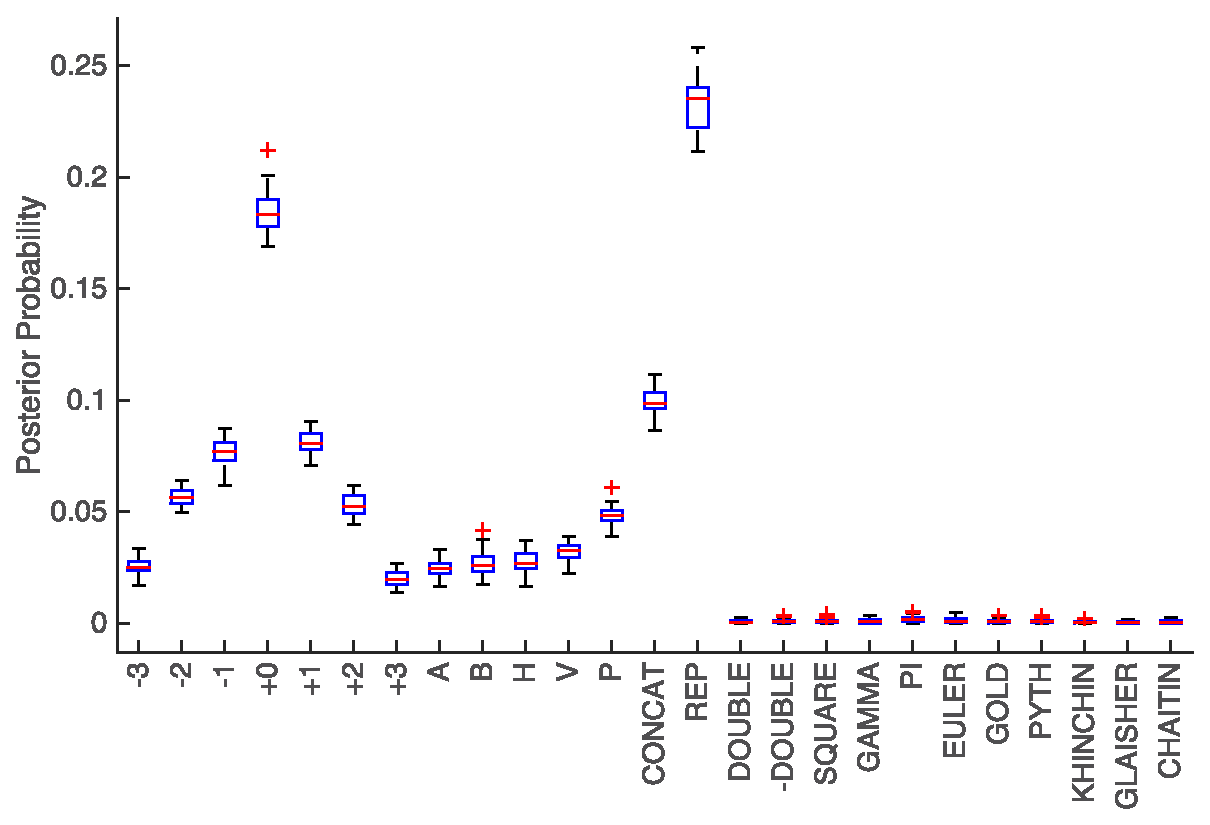
\includegraphics[width=0.8\textwidth]{Fig2}
    %\caption{\bf{Inferred $\theta_i$.} Inferred probability for each production in the grammar}
    \caption{$\theta_i$ inferido. Probabilidad inferida para cada producción de la gramática}
    \label{fig:inferredtheta}
\end{figure}

Aunque 50 pasos puedan parecer pocos para que converja un algoritmo de MCMC, nuestro método calculó $P(p_i \mid d_i, \theta)$ de manera exacta para acelerar la convergencia y para poder luego comparar la probabilidad con la complejidad \mdlgeo del modelo original. En la Figura~\ref{fig:convergetheta}, mostramos una traza de ejemplo para cuatro ejecuciones de MCMC para $\theta_{{\tt +0}}$, que corresponde al valor atómico de la producción \verb#+0#, pero es representativo del comportamiento de todos los $\theta_i$. (consultar la Figura~\ref{S1_Fig} para las trazas del conjunto entero de producciones).

\begin{figure}[htpb]
    \centering
    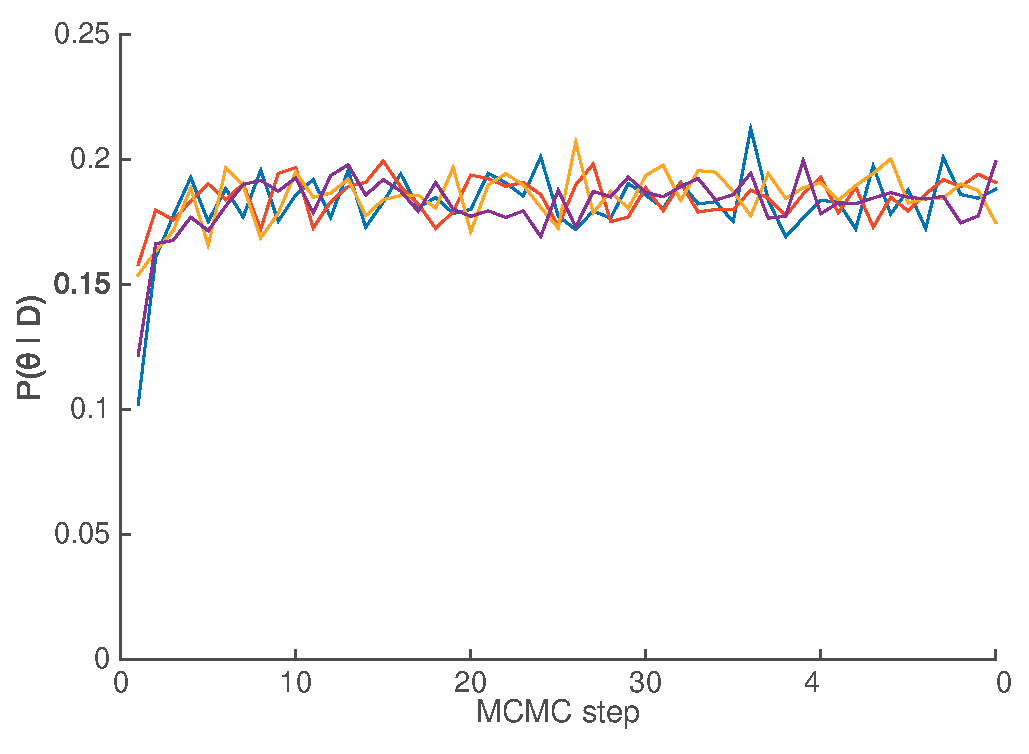
\includegraphics[width=0.8\textwidth]{Fig3}
    %\caption{{\bf Inferred $\theta_{\text{+0}}$.} Inferred probability for +0 production at each step in four MCMC chains.}
    \caption{$\theta_{{\tt +0}}$ inferido. Probabilidad inferida para {\tt +0} en cada paso para cuatro cadenas de MCMC.}
    \label{fig:convergetheta}
\end{figure}

%Figura~\ref{fig:inferredtheta} shows a remarkable difference between the probability of the productions that were originally used based on geometrical intuitions and the ad-hoc productions. The plot also shows that each clockwise production has almost the same probability as its corresponding anticlockwise production, and a similar relation appears between horizontal and vertical symmetry (H and V) and symmetries around diagonal axes (A and B). This is important because the original experiment was designed to balance such behavior; the inferred grammar reflects this.

La Figura~\ref{fig:inferredtheta} muestra una diferencia notable entre la probabilidad de las producciones que se utilizaron originalmente sobre la base de intuiciones geométricas y las producciones ad-hoc. El gráfico muestra también que cada producción en el sentido horario tiene casi la misma probabilidad que su correspondiente producción en sentido antihorario, y una relación similar aparece entre la simetría horizontal y la vertical (\verb#H# y \verb#V#) y las simetrías alrededor de los ejes diagonales (\verb#A# y \verb#B#). Esto es importante porque el experimento original fue diseñado para equilibrar tal comportamiento y la gramática inferida lo refleja también.

%Figura~\ref{fig:thetaGrouped} shows the same inferred $\theta$ but grouped according to production family. Grouping stresses the low probability of all the ad-hoc productions, but also shows an important difference between REP and the rest of the productions, particularly the simple concatenation of productions (CONCAT). This indicates that the \textit{language of geometry} is capable of reusing simpler structures that capture geometrical meaning to explain the observed data, a key aspect of a successful model of LoT.

La Figura~\ref{fig:thetaGrouped} muestra el mismo $\theta$ inferido pero agrupado según su familia de producción. El agrupamiento destaca la baja probabilidad de todas las producciones ad-hoc, pero también muestra una diferencia importante entre \verb#REP# y el resto de las producciones, particularmente respecto de la simple concatenación de producción (\verb#,#). Esto indica que el lenguaje de geometría es capaz de reutilizar estructuras más simples que capturan el significado geométrico para explicar los datos observados, un aspecto clave de un modelo exitoso de \lot que también se ve reflejado en la gramática inferida.

\begin{figure}[!ht]
    \centering
    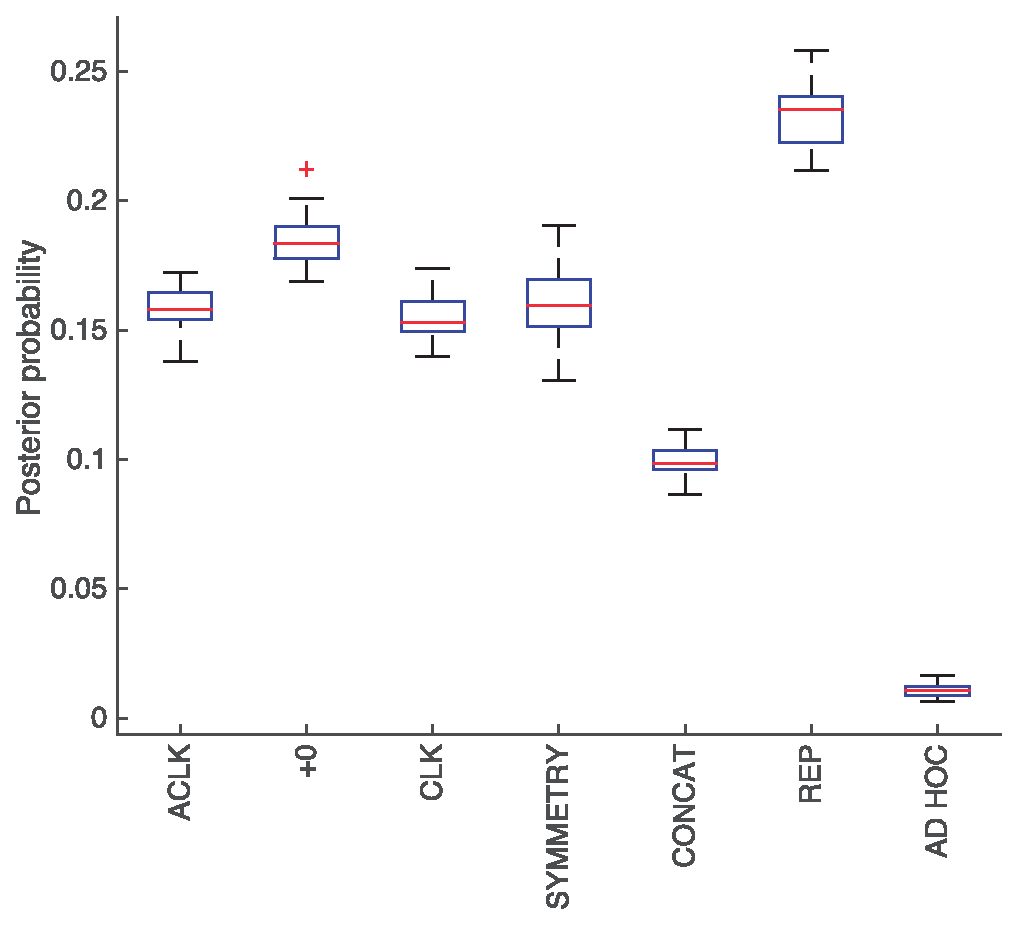
\includegraphics[width=0.8\textwidth]{Fig4}
    \caption{$\theta_i$ inferido agrupado por familia. Probabilidad inferida para cada producción en \gramgeoprima, agrupada por familia.}
    \label{fig:thetaGrouped}
\end{figure}

%We then ran the same inference method using observed sequences from other experiments but only with the original grammar productions (i.e.\ setting aside the ad-hoc productions). We compared the result of inferring over our previously analyzed sequences generated by adults with sequences generated by children (experiment 2 from ~\cite{amalric2017language}) and the actual expected sequences for an ideal player.

Luego ejecutamos el mismo método de inferencia utilizando las secuencia observadas en otros experimentos, pero sólo con las producciones gramaticales originales (es decir, dejando de lado las producciones ad-hoc). Comparamos el resultado de inferir sobre nuestras secuencias previamente analizadas (que habían sido generadas por adultos) con aquellas generadas por niños (el Experimento 2 de~\cite{amalric2017language}) y con las secuencias esperadas para un jugador ideal, es decir, un jugador que siempre elige para cada secuencia $s$ un programa $p$ tal que $\mdlgeo(s) = |p|$ y $\sem{p}=s$ con probabilidad uniforme entre todos los programas mínimos para esa secuencia.

%Figura~\ref{fig:adultVsChildren} shows the probabilities for each atomic production that is inferred after each population. The figure denotes that different populations can converge to different probabilities and thus different LoTs. Specifically, it is worth mentioning that the ideal learner indeed uses more repetition productions than simple concatenations when compared to adults. In the same way, adults use more repetitions than children. This could mean that the ideal learner is capable of reproducing the sequences by recursively embedding other smaller programs, whereas adults and children more so have problems understanding or learning the smaller concept that can explain all the sequences from the experiments, which is consistent with the results from the MDL model in~\cite{amalric2017language}.

La Figura~\ref{fig:adultVsChildren} muestra las probabilidades para cada producción atómica que se infieren de los datos de cada población. La figura denota que diferentes poblaciones pueden converger a diferentes probabilidades y, por tanto, a diferentes LoTs. Específicamente, vale la pena mencionar que el sujeto ideal de hecho utiliza más producciones de repetición que simples concatenaciones en comparación con los adultos. Del mismo modo, los adultos utilizan más repeticiones que los niños. Esto podría significar que el sujeto ideal es capaz de reproducir las secuencias reutilizando de manera recursiva otros programas más cortos, mientras que los adultos y los niños tienen más problemas para comprender o aprender el programa más corto que puede explicar cada una de las secuencias de los experimentos, lo cuál es consistente con los resultados del modelo original de~\cite{amalric2017language}.

\begin{figure}[!ht]
    \centering
    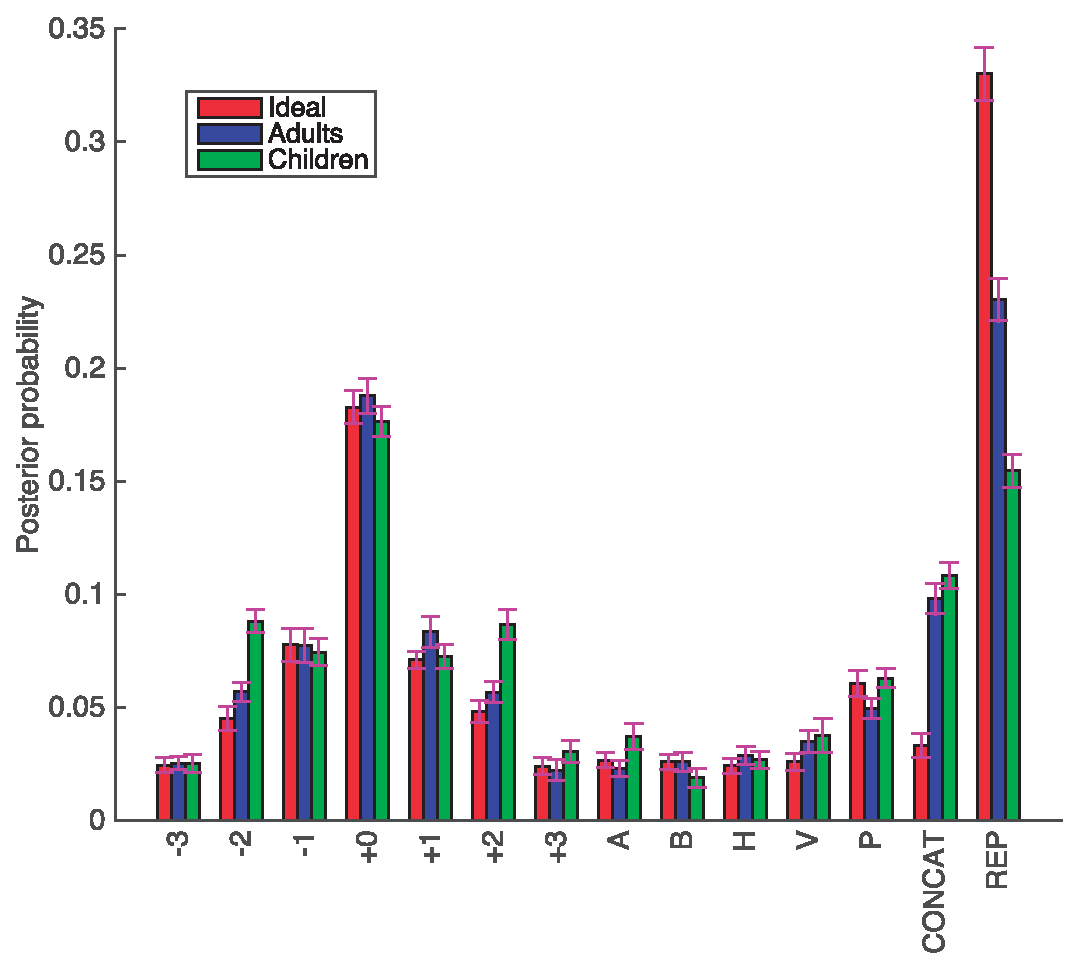
\includegraphics[width=0.8\textwidth]{Fig5}
    %\caption{{\bf Inferred $\theta_i$ for ideal learner, adults and children.} Inferred probability for each production in the grammar for different population data.}
    \caption{$\theta_i$ inferido para el jugador ideal, adultos y niños. Probabilidad inferida para cada producción de \gramgeo para las diferentes poblaciones.}
    \label{fig:adultVsChildren}
\end{figure}

%It is worth mentioning that in~\cite{amalric2017language} the complete grammar for the \textit{language of geometry} could explain adults' behavior but had problems to reproduce the children's patterns for some sequences. However, they also showed that penalizing the rotational symmetry (P) could adequately explain children's behavior. In Figura~\ref{fig:adultVsChildren}, we see that the mean value of (P) for children is 0.06 whereas in adults it's 0.05 (a two-sample t-test reveals t = -12.6, p = 10-19). This might not necessarily be contradictory, as the model for children in~\cite{amalric2017language} was used to predict the next symbol of a sequence after seeing its prefix by adding a penalization for extensions that use the rotational symmetry in the {\em minimal} program of each sequence. On the other hand, the Bayesian model in this work tries to explain the observed sequences produced by children considering the probability of a sequence summing over {\em all} the possible programs that can generate it and not just the ones with minimal size. Thus, a production like (P) that might not be part of the minimal program for a sequence might not necessarily be less probable when considering the entire distribution of programs for that same sequence.

Cabe mencionar que en~\cite{amalric2017language} la gramática completa para el \textit{lenguaje de geometría} podía explicar el comportamiento de los adultos, pero tenía problemas para reproducir los patrones de los niños para algunas secuencias. Sin embargo, también demostraron que penalizar a la simetría rotacional (instrucción atómica \verb#P#)  podría explicar adecuadamente el comportamiento de los niños. En la Figura~\ref{fig:adultVsChildren}, vemos que el valor medio de \verb#P# para niños es 0.06 mientras que en adultos es 0.05 (un t-test de dos muestras revela que $t = -12.6, p = 10^{-19}$). Esto puede no ser necesariamente contradictorio, ya que el modelo para niños en~\cite{amalric2017language} fue utilizado para predecir el siguiente símbolo de una secuencia después de ver su prefijo agregando una penalización para extensiones que usan la simetría rotacional \verb#P# \textit{en el programa mínimo} de cada secuencia. Por otro lado, el modelo bayesiano en este trabajo intenta explicar las secuencias observadas producidas por los niños considerando la probabilidad de una secuencia a partir de sumar todos los posibles programas que la pueden generar \textit{y no sólo en los de tamaño mínimo}. Así, una producción como \verb#P# que podría no ser parte del programa mínimo para una secuencia, puede no ser necesariamente menos probable cuando se considera la distribución total de programas para esa misma secuencia.

%\section{Coding Theorem}
\section{Teorema de codificación}
\label{sec:coding}

%For each phenomenon there can always be an extremely large, possibly infinite, number of explanations. In a LoT model, this space is constrained by the grammar $\gram$ that defines the valid hypotheses in the language. Still, one has to define how a hypothesis is chosen among all possibilities. Following Occam's razor, one should choose the simplest hypothesis amongst all the possible ones that explain a phenomenon. In cognitive science, the MDL framework has been widely used to model such bias in human cognition, and in \textit{the language of geometry} in particular~\cite{amalric2017language}. The MDL framework is based on the ideas of information theory~\cite{shannon48}, Kolmogorov complexity~\cite{kolmogorov1968three} and Solomonoff induction~\cite{solomonoff1964formal}.

Para cada fenómeno siempre puede haber un número extremadamente grande, posiblemente infinito, de explicaciones. En un modelo de \lot, este espacio está limitado por la gramática $\gram$ que define las hipótesis válidas en el lenguaje. Aún así, hay que definir cómo se elige una hipótesis entre todas las posibles. Siguiendo el principio de la navaja de Ockham, se debe elegir la hipótesis más simple entre todas las posibles que explican un fenómeno. En ciencia cognitiva, y en \gramgeo en particular, se suele utilizar nociones basadas en el principio de longitud mínima de descripción como \mdlgeo para modelar tal sesgo en la cognición.

%Occam's razor was formalized by Solomonoff~\cite{solomonoff1964formal} in his theory of universal inductive inference, which proposes a universal prediction method that successfully approximates any distribution $\mu$ based on previous observations, with the only assumption of $\mu$ being computable. In short, Solomonoff's theory uses all programs (in the form of prefix Turing machines) that can describe previous observations of a sequence to calculate the probability of the next symbols in an optimal fashion, giving more weight to shorter programs. Intuitively, simpler theories with low complexity have higher probability than theories with higher complexity. Formally, this relationship is described by the Coding Theorem~\cite{levin1974laws}, which closes the gap between the concepts of Kolmogorov complexity and probability theory. However, LoT models that define a probabilistic distribution for their hypotheses do not attempt to compare it with a complexity measure of the hypotheses like the ones used in MDL, nor the other way around.

El principio de la navaja de Ockham fue formalizado por Solomonoff~\cite{solomonoff1964formal} en su teoría universal de la inferencia inductiva, que propone un método de predicción universal que aproxima cualquier distribución $\mu$ a partir de observaciones previas, con el único supuesto de que $\mu$ sea computable. En resumen, la teoría de Solomonoff utiliza todos los programas (en la forma de máquinas de Turing libres de prefijos) que pueden describir las observaciones previas de una secuencia para calcular la probabilidad de los siguientes símbolos de una manera óptima, dando más peso a los programas más cortos. Intuitivamente, las teorías más simples, con baja complejidad, tienen mayor probabilidad que las teorías de mayor complejidad. Formalmente, esta relación es descrita en el Teorema de codificación~\cite{levin1974laws}, que cierra la brecha entre los conceptos de complejidad de Kolmogorov y la teoría de probabilidad. Sin embargo, los modelos de \lot que definen una distribución probabilística para sus hipótesis no han intentado compararla con una medida de complejidad de las hipótesis (como las que se usan en \mdlgeo), ni al revés.

%In what follows we formalize the Coding Theorem (for more information, see~\cite{li2013introduction}) and test it experimentally. To the best our knowledge, this is the first attempt to validate these ideas for a particular (non universal) language. The reader should note that we are not validating the theorem itself as it has already been proved for universal Turing Machines. Here, we are testing whether the inverse logarithmic relationship between the probability and complexity holds true when defined for a specific non universal language.

A continuación, formalizamos el Teorema de Codificación (para obtener más información, consultar~\cite{li2013introduction}) y lo probamos experimentalmente. Hasta donde sabemos, este es el primer intento para validad estas ideas para un lenguaje particular (no universal). El lector debe tener en cuenta que no estamos validando el teorema en sí, dado que ha sido postulado y probado para máquinas de Turing {\em universales}. Aquí estamos probando si la relación logarítmica inversa entre la probabilidad y la complejidad podría mantenerse cuando se definen para un lenguaje específico no universal.

%\subsection{The formal statement}
\subsection{La definición formal}

%Let $M$ be a prefix Turing machine --by {\em prefix} we mean that if $M(x)$ is defined, then $M$ is undefined for every proper extension of $x$. Let $P_M(x)$ be the probability that the machine $M$ computes output $x$ when the input is filled-up with the results of fair coin tosses, and let $K_M(x)$ be the {\em Kolmogorov complexity of $x$ relative to $M$}, which is defined as the length of the shortest program which outputs $x$, when executed on $M$. The Coding Theorem states that for every string $x$ we have


Para avanzar en la definición del Teorema de Codificación, necesitaremos primero introducir las máquinas de Turing {\em libres de prefijos}~\cite{L71,L73,S71,chaitin1975theory}. Desde el punto de vista de la arquitectura, este dispositivo es análogo a una máquina de Turing clásica, pero la cinta de entrada es un poco más primitiva: el cabezal de entrada se mueve solo hacia la derecha y no hay un blanco al final u otra marcador que delimite el final de la entrada. De esta manera, una máquina libre de prefijos que comienza con el cabezal de entrada en el primer bit de la entrada, puede eventualmente intentar leer más allá del final y, si esto sucede, simplemente falla (es decir, se indefine) y permanece en ese estado de error para siempre. Por lo tanto, para que una máquina libre de prefijos $\M$ tenga éxito en el cálculo, necesita averiguar por sí misma dónde está el final de la entrada. Esta es la razón por la que este dispositivo a veces recibe el nombre de máquina {\em autodelimitante}. En este modelo, si se define una entrada dada, todas sus extensiones son indefinidas. Se puede demostrar que esta arquitectura restringida de máquinas de Turing calcula exactamente todas las funciones computables parciales con dominio libre de prefijos. La complejidad libre de prefijos de Kolmogorov~\cite{levin1974laws,G74,chaitin1975theory} se define de la misma manera que en la Definición \ref{intro:def:plainC} pero relativa a máquinas libres de prefijos.


\begin{definicion}[Conjunto libre de prefijos]\label{seleccion:def:conjuntolibreprefijos}
Para
$\sta,\stb\in\words$, escribimos
\glossary{$\preceq$}$\sta\preceq\stb$ cuando $\sta$ es un prefijo de
$\stb$, es decir, $\len{\sta}\leq\len{\stb}$ y $\sta(i)=\stb(i)$
para todo $i\in\{0,\dots,\len{\sta}-1 \}$. Utilizamos
\glossary{$\prec$}$\sta\prec\stb$ cuando $\sta$ es un prefijo propio de $\stb$, es decir, $\sta\preceq \stb$ y $\sta\not=\stb$. Un conjunto de cadenas $A$ es {\em libre de prefijos} si no hay dos cadenas $\sta$
y $\stb$ en $A$ tal que $\sta\prec\stb$. 
%Un conjunto $T\subseteq\words$ es un \index{tree} {\em árbol} si para todo $\sta,\stb\in\words$ si $\sta\in T$ y $\stb\prec\sta$ entonces $\stb\in T$.
\end{definicion}

\begin{definicion}[Complejidad de Kolmogorov libre de prefijos]\label{seleccion:def:prefixK}
\glossary{$\KM$}$\KM\colon\words \to \nat$, la complejidad de Kolmogorov libre de prefijos con respecto a la máquina $\M$ libre de prefijos se define como:
$$
\KM(\sta)=
    \begin{cases}
    \min \{\len{\pra}\colon \M(\pra)=\sta \} & \textrm{si $\sta$ en el rango de $\M$};\\
    \infty & \textrm{sino}
    \end{cases}
$$
\end{definicion}


%There are two traditions of notation in the \kolcomp community as regards the plain/\pfree versions: the $C$/$K$ tradition and the $K$/$H$ tradition. In recent years it seems that the $C$/$K$ notation appears more often in both the complexity and the recursion theory literature. In this document, we follow the $C$/$K$ notation.


%Observe that it does not matter if the list in (\ref{intro:eqn:enumPRfunctions}) is an enumeration of all classical machines or all \pfree machines (both have a finite table of instructions, so they can be effectively listed). The machine $\V$ defined in (\ref{intro:eqn:usualUniversalMachine}) exists in both cases and in the second, $\V$ is also \pfree.


%The classical notion of universality from computability theory is redefined in the algorithmic information theory. We will use the word {\em \opt} for denoting machines like $\V$ defined in(\ref{intro:eqn:usualUniversalMachine}) that somehow simulate every other machine at no noticeable extra cost in the length.

La misma definición \ref{intro:def:optimal} de universalidad dada en aplica a las máquinas libre de prefijos, y, al igual que con las máquinas usuales, existen máquinas universales libres de prefijos. Del mismo modo, el Teorema \ref{intro:thm:invariance} de invariancia también sigue valiendo para el universo de las máquinas libres de prefijos. Cuando $\M$ es una máquina libre de prefijos universal, hablaremos directamente de complejidad de Kolmogorov libre de prefijos y la denotaremos como $\K$. La complejidad $\K$ está relacionada con la probabilidad de que una máquina libre de prefijos produzca una cadena dada. Esta probabilidad se define como \glossary{$P$}:
%
\begin{eqnarray}
P_{\M}(\sta)&=&\measure{\open{\{\pra\colon\M(\pra)=\sta\}}}\nonumber\\
&=&\sum_{\pra\colon\M(\pra)=\sta}2^{-\len{\pra}}, \label{intro:eqn:coding}
\end{eqnarray}
%
en donde $\mu$ es la medida de Lebesgue sobre el espacio de Cantor $2^\omega$, esto es sobre el conjunto de todas las secuencias de ceros y unos infinitas.
Para todo $\sta$, podemos ver que $2^{-\K(\sta)}\leq P_{\U}(\sta)$, ya que una de las $\U$-descripciones de $\sta$ será la de mejor longitud, es decir que tendrá longitud igual a $\K(\sta)$. El siguiente resultado, conocido como el Teorema de la Codificación \cite{levin1974laws,G74,chaitin1975theory}, establece que la otra desigualdad también es verdadera, excepto por una constante multiplicativa.
%
\begin{teorema}[\index{Coding Theorem}Teorema de Codificación]\label{intro:thm:coding} Para cada máquina libre de prefijos $\M$se puede obtener efectivamente una constante $c$ tal que $ (\forall
\sta\in\words)\ 2^{c-\K(\sta)}\geq P_{\M}(\sta). $
\end{teorema}
%
Así, cuando $\M=\U$, obtenemos que $P_{\U}$ y $2^\K$ son proporcionales. Para más información sobre el Teorema de Codificación, se puede consultar \cite{li2013introduction,DHBook}.

%\index{Program-size complexity@\kolcomp!\computable@\comp approximation} Although $\K$ and $\C$ are not \comp functions, they can be \recly approximated from above using the step by step approximation of $\U$. \glossary{$\K_s$}$\K_s(\sta)$ is the approximation at stage $s$ of $\K(\sta)$ defined by $\K_s(\sta)=\min\{\len{\pra}\colon \U_s(\pra)=\sta\}\cup\{\infty\}$. Observe that $\K_s(\sta)\to\K(\sta)$ when $s\to\infty$. The same holds for \glossary{$\C_s$}${\C_s}$.

%Machines can be relativized to oracles. For any $\M^A$, a \pfree machine $\M$ relativized to an oracle $A$, $\domain {\M^A}$ has to be \pfree. The Definition~\ref{intro:def:prefixK} of \kolcomp can be relativized to oracles:

%\begin{definicion}[Relativized \pfree \kolcomp]\label{intro:def:prefixKwithOracle}
%\index{Program-size complexity@\kolcomp!relativized} \glossary{$\KM^A$}$\KM^A\colon\words \to \nat$, the {\em \pfree \kolcomp with respect to the \pfree machine $\M$ and relative to oracle $A$}, is defined as
%$$
%\KM^A(\sta)=
%    \begin{cases}
%    \min \{\len{\pra}\colon \M^A(\pra)=\sta \} & \textrm{if $\sta$ is in the range of $\M^A$};\\
%    \infty & \textrm{otherwise.}
%    \end{cases}
%$$
%\end{definicion}

%Definition~\ref{intro:def:plainC} of $\CM$ also adapts straightforwardly to \glossary{$\CM^A$}$\CM^A$. Again, when there is no need to refer to the underlying \opt machine, we just write \glossary{$\C^A$}$\C^A$ and \glossary{$\K^A$}$\K^A$. Having an oracle $A$ gives more power for compressing strings, so $\K^A$ is always smaller than $\K$ up to an additive constant. The same holds for $\C^A$ and $\C$.

%Sea $M$ una Máquina de Turing libre de prefijos --por {\em libre de prefijo} nos referimos a que si $M(x)$ está definida, entonces $M$ está indefinida para cualquier extensión de $x$. Sea $P_M(x)$ la probabilidad de que la máquina $M$ compute la salida $x$ cuando la entrada se llena con los resultados de los lanzamientos de una moneda justa, y sea $K_M(x)$ la {\em complejidad de Kolmogorov de $x$ relativa a $M$}, que se define como la longitud del programa más corto que genera $x$, cuando se ejecuta en $M$. El Teorema de Codificación establece que, por cada cadena $x$ tenemos:
%
%\begin{equation*}
%\label{eqF}
%\log \frac{1}{P_U(x)} = K_U(x)
%\end{equation*}
%
%up to an additive constant, whenever $U$ is a {\em universal} prefix Turing machine --by {\em universal} we mean a machine which is capable of simulating every other Turing machine; it can be understood as the underlying (Turing-complete) chosen programming language. It is important to remark that neither $P_U$, nor $K_U$ are computable, which means that such mappings cannot be obtained through effective means. However, for specific (non-universal) machines $M$, one can, indeed, compute both $P_M$ and $K_M$.
%salvo una constante aditiva, siempre que $U$ sea una Máquina Universal de Turing libre prefijos --por {\em Universal} nos referimos a una máquina que es capaz de simular cualquier otra máquina de Turing; puede entenderse como el lenguaje de programación elegido subyacente (Turing-completo). Es importante señalar que ni $P_U$, ni $K_U$ son computables, lo que significa que tal mapeo no puede obtenerse por medios efectivos. Sin embargo, para máquinas específicas (no universales) $M$, uno puede, de hecho, calcular tanto $P_M$ como $K_M$.

%\subsection{Testing the Coding Theorem for \boldmath{$\gramgeo$}}
\subsection{Revisando el teorema de codificación para \gramgeo}

%Despite the fact that $P_M$ and $K_M$ are defined over a Turing Machine $M$, the reader should note that a LoT is not usually formalized with a Turing Machine, but instead as a programming language with its own syntax of valid programs and semantics of execution, which stipulates how to compute a concept from a program. However, one can understand programming languages as defining an equivalent (not necessarily universal) Turing Machine model, and a LoT as defining its equivalent (not necessarily universal) Turing Machine $\gram$. In short, machines and languages are interchangeable in this context: they both specify the programs/terms, which are symbolic objects that, in turn, describe semantic objects, namely, strings.

A pesar de que $P_{\M}$ y $K_{\M}$ están definidos sobre una máquina de Turing $\M$, el lector debe tener en cuenta que un \lot no se suele formalizar con una máquina de Turing, sino como un lenguaje de programación con su propia sintaxis de programas válidos y su propia semántica de ejecución que estipula cómo calcular un concepto a partir de un programa válido. Sin embargo, uno puede concebir los lenguajes de programación como la definición de una máquina de Turing equivalente (no necesariamente universal), y a un \lot como un lenguaje que define a su equivalente máquina de Turing (no necesariamente universal), En resumen, las máquinas y los lenguajes son intercambiables en este  sentido: ambas especifican los programas/términos, los cuales son objetos simbólicos que, a su vez, describen objetos semánticos (a saber, cadenas). Para \gramgeo ya tenemos definida su medida de $K_{\M}$ a la cual hemos notado \mdlgeo, a continuación definiremos $P_{\M}$ para el mismo lenguaje.

%\paragraph{The Kolmogorov complexity relative to \boldmath{$\gramgeo$}}

%In~\cite{amalric2017language}, the Minimal Description Length was used to model the combination of productions from the \textit{language of geometry} into concepts by defining a Kolmogorov complexity relative to the {\em language of geometry}, which we denote $\mdlgeo$. $\mdlgeo(x)$ is the minimal size of an expression in the grammar of $\gramgeo$ which describes $x$. The formal definition of `size' can be found in the cited work but in short: each of the atomic productions adds a fixed cost of $2$ units; using any of the repetition productions to iterate $n$ times a list of other productions adds the cost of the list, plus $\lfloor \log(n) \rfloor$; and joining two lists with a concatenation costs the same as the sum of the costs of both lists.


%\paragraph{The probability relative to \boldmath{$\gramgeo$}} On the other hand, with the Bayesian model specified in this work, we can define $P(x \mid \gramgeo, \theta)$ which is the probability of a string $x$ relative to $\gramgeo$ and its vector of probabilities for each of the productions.

\paragraph{La probabilidad relativa \gramgeo.} 

Con el modelo bayesiano especificado en este capítulo podemos definir $P(x \mid \gramgeo, \theta)$ que es la probabilidad de una cadena $x$ relativa a \gramgeo y el vector de probabilidades para cada una de las producciones.

%For the sake of simplicity, we will use $P_{\gramgeo}(x)$ to denote $P(x \mid \gramgeo, \theta)$ when $\theta$ is the inferred probability from the observed adult sequences from the experiment.
En aras de la simplicidad, usaremos $P_{\gramgeo}(x)$ para denotar $P(x \mid \gramgeo, \theta)$ cuando $\theta$ es la probabilidad inferida de las secuencias de adultos observadas en el experimento:
%
\begin{eqnarray*}
\label{eqG}
P_{\gramgeo}(x) &=& P(x \mid \gramgeo, \theta)\\
&=& \sum_{\prog} P(x \mid \prog, \theta)\\
&\propto &\sum_{\prog} P(x \mid \prog) P(\prog \mid \theta).
\end{eqnarray*}
%

%Here, we calculate both $P_{\gramgeo}(x)$ and $K_{\gramgeo(x)}$ in an exact way (note that $\gramgeo$, seen as a programming language, is not Turing-complete). In this section, we show an experimental equivalence between such measures which is consistent with the Coding Theorem. We should stress, once more, that the theorem does not predict that this relationship should hold for a specific non-universal Turing Machine.

Aquí, calculamos tanto $P_{\gramgeo}(x)$ como $\mdlgeo(x)$ de una manera efectiva (tener en cuenta que \gramgeo, visto como un lenguaje de programación, no es Turing-completo). En esta sección, mostramos un experimento de equivalencia entre tales medidas que es consistente con el Teorema de Codificación. Queremos enfatizar, una vez más, que el teorema no predice que esta relación deba mantenerse para una máquina de Turing específica, no universal.


%To calculate $P_{\gramgeo}(x)$ we are not interested in the normalization factor of $P(x \mid \prog) P(\prog \mid \theta)$ because we are just trying to measure the relationship between $P_{\gramgeo}$ and $\mdlgeo$ in terms of the Coding Theorem. Note, however, that calculating $P_{\gramgeo}(x)$ involves calculating all programs that compute each of the sequences as in our previous experiment. To make this tractable we calculated $P_{\gramgeo}(x)$ for 10,000 unique random sequences for each of the possible sequence lengths from the experiment (i.e., up to eight). When the length of the sequence did not allow 10,000 unique combinations, we used all the possible sequences of that length.

Para calcular $P_{\gramgeo}(x)$ no nos interesa el factor de normalización de $P(x \mid \prog) P(\prog \mid \theta)$ porque sólo estamos tratando de medir la relación entre $P_{\gramgeo}$ y $\mdlgeo$ en términos del Teorema de Codificación. Sin embargo, hay que tener en cuenta que el cálculo de $P_{\gramgeo}(x)$ implica calcular todos los programas que computan cada una de las secuencias como en nuestro experimento anterior. Para hacer esto tratable, calculamos $P_{\gramgeo}(x)$ para 10.000 secuencias aleatorias únicas para cada una de las posibles longitudes de las secuencias del experimento (es decir, hasta ocho). Cuando la longitud de la secuencia no permitió 10.000 combinaciones únicas, utilizamos todas las posibles secuencias de esa longitud.

%\subsection{Coding Theorem Results}
\subsection{Resultados del Teorema de Codificación}

%Figura~\ref{fig:codR} shows the mean probability $P_{\gramgeo}(x)$ for all sequences $x$ with the same value of $K_{\gramgeo(x)}$ and length between 4 and 8 ($|x| \in \left[4,8 \right]$) for all generated sequences $x$. The data is plotted with a logarithmic scale for the x-axis, illustrating the inverse logarithmic relationship between $\mdlgeo(x)$ and $P_{\gramgeo}(x)$. The fit is very good, with $R^2=.99$, $R^2=.94$, $R^2=.97$, $R^2=.99$ and $R^2=.98$ for Figura~\ref{fig:codR}A, Figura~\ref{fig:codR}B, Figura~\ref{fig:codR}C, Figura~\ref{fig:codR}D and Figura~\ref{fig:codR}E, respectively.

La Figura~\ref{fig:codR} muestra la probabilidad media $P_{\gramgeo}(x)$ para todas las secuencias $x$ con el mismo valor de $\mdlgeo(x)$ y una longitud entre 4 y 8 ($|x| \in \left[4,8 \right]$) para todas las secuencias generadas $x$. Los datos se trazan con una escala logarítmica para el eje x, ilustrando la relación logarítmica inversa entre $\mdlgeo(x)$ y $P_{\gramgeo}(x)$. El ajuste es muy bueno, con $R^2=.99$, $R^2=.94$, $R^2=.97$, $R^2=.99$ y $R^2=.98$ para Figura~\ref{fig:codR}A, Figura~\ref{fig:codR}B, Figura~\ref{fig:codR}C, Figura~\ref{fig:codR}D y Figura~\ref{fig:codR}E, respectivamente.

\begin{figure}[!ht]
    \centering
    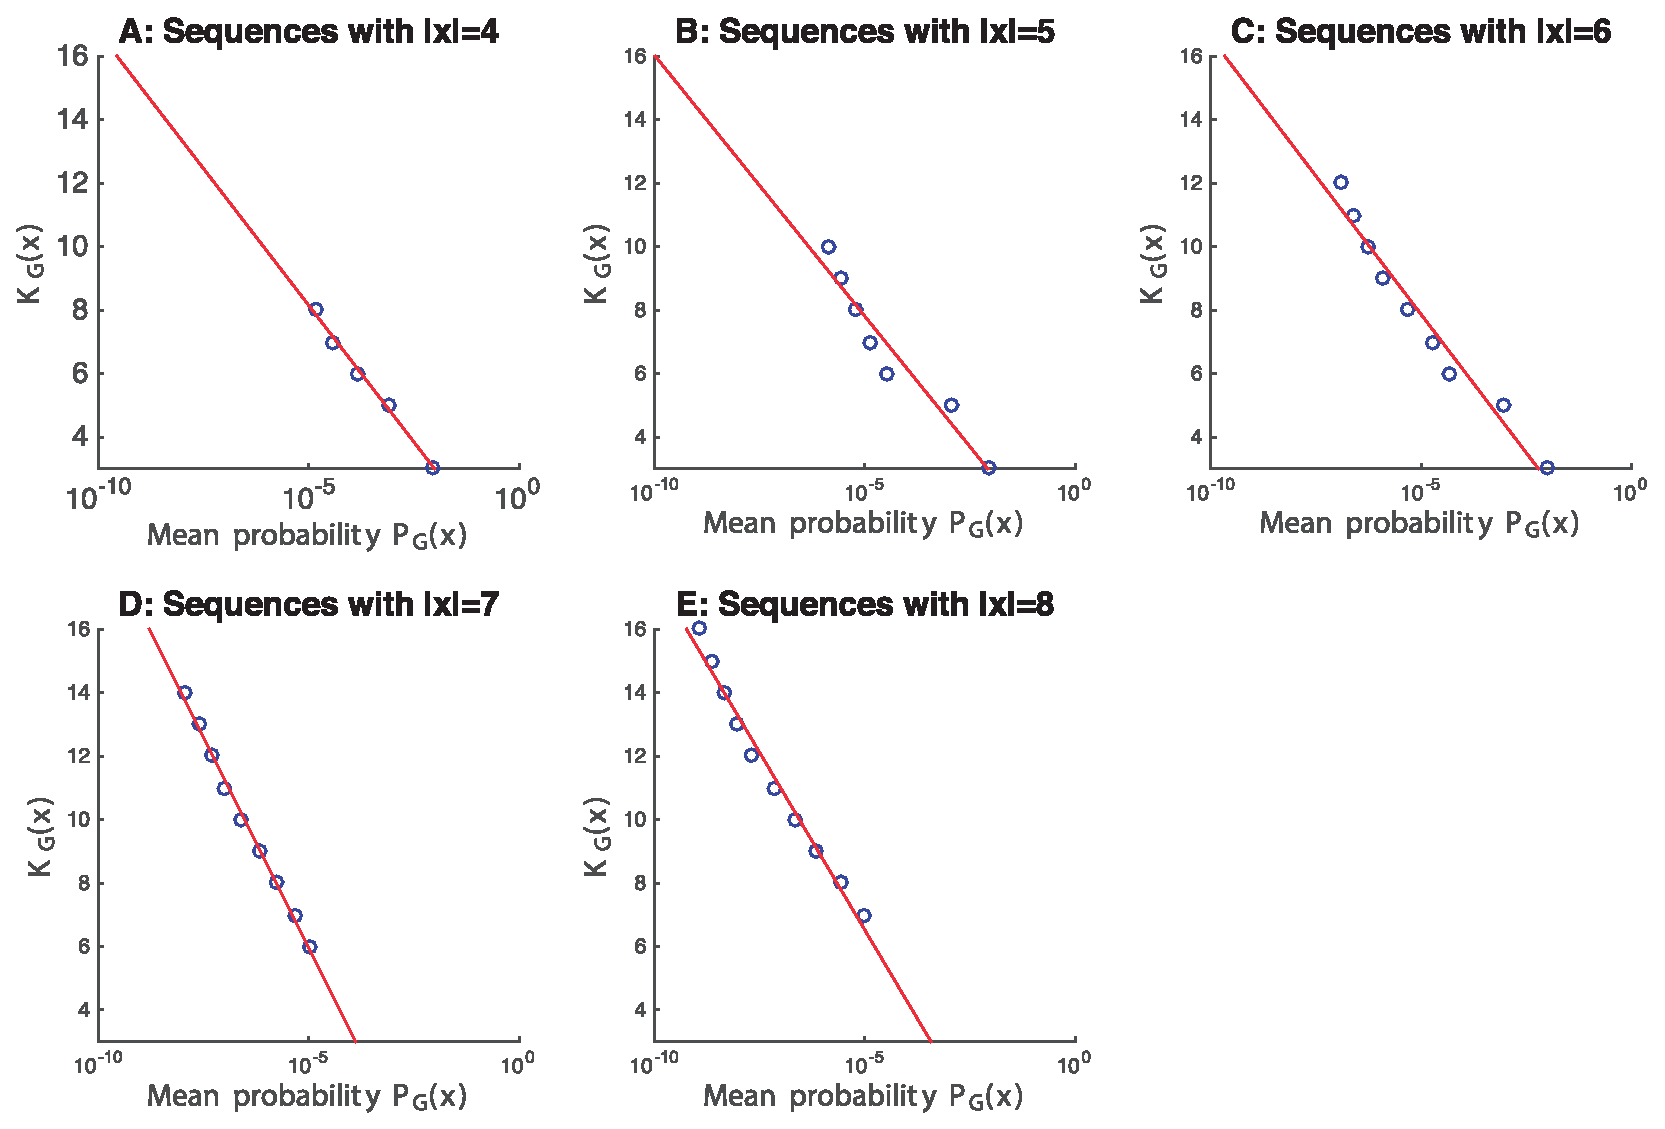
\includegraphics[width=1\textwidth]{Fig6}
    \caption{Probabilidad media $P_{\gramgeo}(x)$ para todas las secuencias $x$ con el mismo valor de $\mdlgeo(x)$.
    Subfigura A: secuencias con $|x| = 4$.
    Subfigura B: secuencias con $|x| = 5$.
    Subfigura C: secuencias con $|x| = 6$.
    Subfigura D: secuencias con $|x| = 7$.
    Subfigura E: secuencias con $|x| = 8$.}
    \label{fig:codR}
\end{figure}

%This relationship between the complexity $\mdlgeo$ and the probability $P_{\gramgeo}$ defined for finite sequences in the \textit{language of geometry}, matches the theoretical prediction for infinite sequences in universal languages described in the Coding Theorem. At the same time, it captures the Occam's razor intuition that the simpler sequences one can produce or explain with this language are also the more probable.

Esta relación entre la complejidad $\mdlgeo$ y la probabilidad $P_{\gramgeo}$ definidas para secuencias finitas en \gramgeo, coincide con al predicción teórica para cadenas en lenguajes universales descrita en el Teorema de Codificación. Al mismo tiempo, captura la intuición de la navaja de Ockham por la cual las secuencias más simples que uno puede producir o explicar en este lenguaje son también las más probables.

%Figura~\ref{fig:codK:8} and Figura~\ref{fig:codP:8} show the histogram of $P_{\gramgeo}(x)$ and $\mdlgeo(x)$, respectively, for sequences with length = 8 to get a better insight about both measures. The histogram of the rest of the sequence's lengths are included in \nameref{S2_Fig} and \nameref{S3_Fig} for completeness, and they all show the same behavior.

En Figura~\ref{fig:codK:8} y Figura~\ref{fig:codP:8} se muestra el histograma de $P_{\gramgeo}(x)$ y $\mdlgeo(x)$, respectivamente, para secuencias de longitud = 8 para obtener una mejor idea de ambas distribuciones. El histograma del resto de las longitudes de la secuencia se incluyen en las Figuras \ref{S2_Fig} y \ref{S3_Fig} del apéndice \ref{app:PO} por completitud, y todos muestran el mismo comportamiento.

\begin{figure}[!ht]
    \centering
    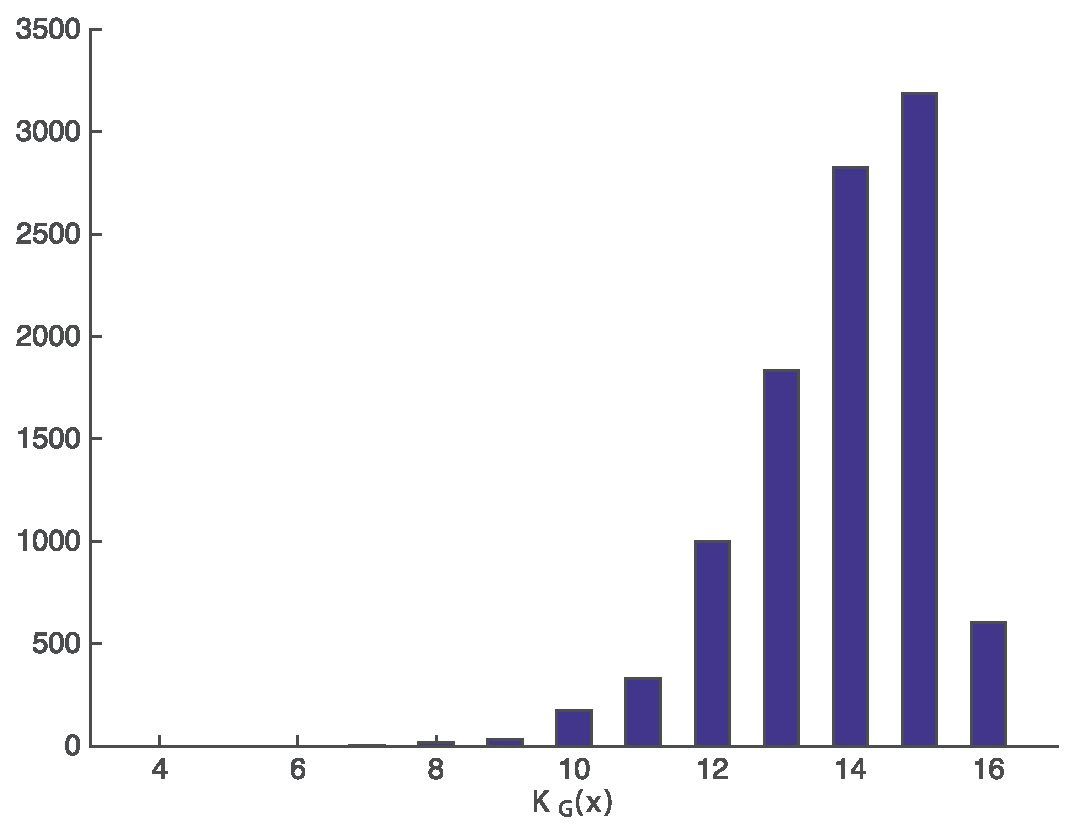
\includegraphics[width=0.8\textwidth]{Fig7}
    %\caption{{\bf Histogram of complexity $\mdlgeo(x)$.} Histogram of complexity for sequences $x$ with $|x| = 8$.}
    \caption{Histograma de complejidad $\mdlgeo(x)$ para secuencias $x$ con $|x| = 8$.}
    \label{fig:codK:8}
\end{figure}


\begin{figure}[!ht]
    \centering
    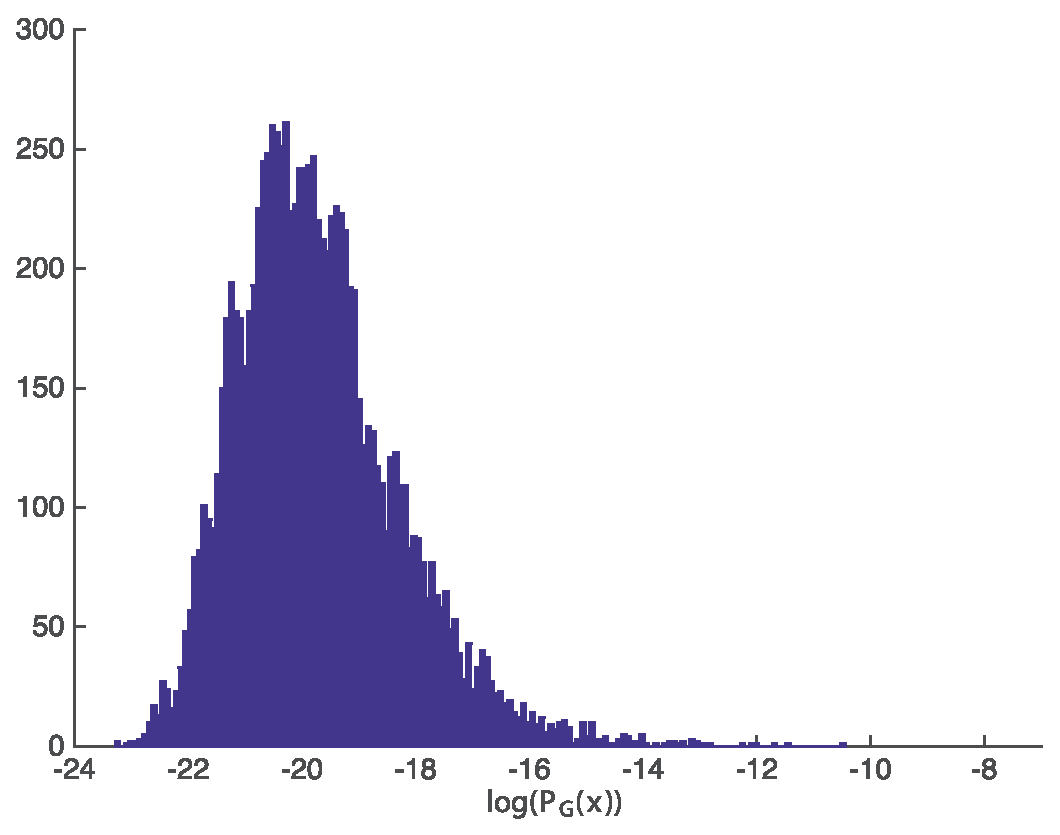
\includegraphics[width=0.8\textwidth]{Fig8}
    %\caption{{\bf Histogram of probability $P_{\gramgeo}(x)$.} Histogram of probability for sequences $x$ with $|x| = 8$.}
    \caption{Histograma de probabilidad $P_{\gramgeo}(x)$ para secuencias $x$ con $|x| = 8$.}
    \label{fig:codP:8}
\end{figure}

%\section{Discussion}
\section{Discusión}

%We have presented a Bayesian inference method to select the set of productions for a LoT and test its effectiveness in the domain of a geometrical cognition task. We have shown that this method is useful to distinguish between arbitrary ad-hoc productions and productions that were intuitively selected to mimic human abilities in such domain.

Hemos presentado un método de inferencia bayesiano para seleccionar el conjunto de producciones para un \lot y probado su eficacia en el dominio de una tarea de cognición geométrica. Mostramos que este método es útil para distinguir entre producciones ad-hoc arbitrarias y producciones que fueron seleccionadas intuitivamente para imitar las habilidades humanas en ese dominio.

%The proposal to use Bayesian models tied to PCFG grammars in a LoT is not new. However, previous work has not used the inferred probabilities to gain more insight about the grammar definition in order to modify it. Instead, it had usually integrated out the production probabilities to better predict the data, and even found that hierarchical priors for grammar productions show no significant differences in prediction results over uniform priors~\cite{piantadosi2012bootstrapping,yildirim2015learning}.

La propuesta de utilizar modelos bayesianos vinculados a gramáticas PCFG en un \lot no es nueva. Sin embargo, los trabajos anteriores no han utilizado las probabilidades inferidas para obtener más información sobre la definición de la gramática y modificarla. En cambio, han integrado usualmente las probabilidades de producción para predecir mejor los datos e incluso se mostró que el uso de distribuciones a priori jerárquicas para las producciones gramaticales no muestran diferencias significativas en los resultados de predicción sobre el uso de distribuciones a priori uniformes~\cite{piantadosi2012bootstrapping,yildirim2015learning}.

%We believe that inferring production probabilities can help prove the adequacy of the grammar, and can further lead to a formal mechanism for selecting the correct set of productions when it is not clear what a proper set should be. Researchers could use a much broader set of productions than what might seem intuitive or relevant for the domain and let the hierarchical Bayesian inference framework select the best subset.

Creemos que inferir probabilidades de producción puede ayudar a demostrar la adecuación de una gramática para un dominio, y puede conducir a un mecanismo formal para seleccionar el conjunto correcto de producciones cuando no está claro cuál debería ser el conjunto correcto. Los investigadores podrían utilizar un conjunto de producciones más amplios que aquellas que parezcan intuitivas o relevantes para el dominio y dejar que la inferencia bayesiana seleccione el mejor subconjunto.

%Selecting a broader set of productions still leaves some arbitrary decisions to be made. However, it can help to build a more robust methodology that --combined with other ideas like testing grammars with different productions for the same task~\cite{piantadosi2016logical}-- could provide more evidence of the adequacy of the proposed LoT.

La selección de un conjunto más amplio de producciones todavía deja algunas decisiones arbitrarias por tomar. Sin embargo, puede contribuir a construir una metodología más sólida que --combinada con otras ideas como probar gramáticas con diferentes producciones para la misma tarea~\cite{piantadosi2016logical}-- podría proporcionar más evidencia de la idoneidad del \lot propuesto.

%Having a principled method for defining grammars in LoTs is a crucial aspect for their success because slightly different grammars can lead to different results, as has been shown in~\cite{piantadosi2016logical}.

Tener un método basado en principios para definir gramáticas en \lot es un aspecto crucial para su éxito, porque gramáticas ligeramente diferentes pueden conducir a resultados muy diversos como se ha demostrado en~\cite{piantadosi2016logical}.

%The experimental data used in this work was designed at~\cite{amalric2017language} to understand how humans encode visuo-spatial sequences as structured expressions. As future research, we plan to perform a specific experiment to test these ideas in a broader range of domains. Additionally, data from more domains is needed to demonstrate if this method could also be used to effectively prove whether different people use different LoT productions as outlined in Figura~\ref{fig:adultVsChildren}.

Los datos experimentales utilizados en este trabajo fueron diseñados en~\cite{amalric2017language} para comprender cómo los humanos codifican secuencias visuoespaciales como expresiones estructuradas. Como investigaciones futuras, podrían realizarse experimentos específicos para probar estas ideas en un rango de dominios más amplios. Además, se necesitan aún más experimentos para probar la efectividad del método y ver si permite individualizar las diferencias de las producciones de los LoTs para distintas poblaciones, como se describió en la Figura~\ref{fig:adultVsChildren}.

%Finally, we showed an empirical equivalence between the complexity of a sequence in a minimal description length (MDL) model and the probability of the same sequence in a Bayesian inference model which is consistent with the theoretical relationship described in the Coding Theorem. This opens an opportunity to bridge the gap between these two approaches that had been described ad complementary by some authors~\cite{mackay2003information}.

Finalmente, mostramos una equivalencia empírica entre la complejidad de una secuencia en un modelo de longitud de descripción mínima y la probabilidad de la misma secuencia en un modelo de inferencia bayesiano, lo cual es consistente con la relación teórica descrita en el Teorema de Codificación dentro de la Teoría de la Información Algorítmica. Esto abre una oportunidad para cerrar la brecha entre estos dos enfoques que han sido descritos como complementarios por algunos autores~\cite{mackay2003information}.

